\exercice \\

\begin{minipage}{0.25\textwidth}
\begin{center}
%\fbox{
\begin{tikzpicture}[scale=1.8,every node/.style={scale=0.7}]
	%Points
	\coordinate(A)at(-1,0);
	\coordinate(B)at(-1,-1);
	\coordinate(C)at(0,-1);
	\coordinate(D)at(0,0);
	\coordinate(E)at(0,1);
	\coordinate(F)at(-1,1);
	\coordinate(G)at(1,0);
	\coordinate(H)at(1,1);
	\coordinate(I)at(2,0);
	\coordinate(J)at(-1,2);
	\draw (A)--(B)--(C)--(D)--cycle;
	\draw (A)--(D)--(E)--(F)--cycle;
	\draw (D)--(G)--(H)--(E)--cycle;
	\draw (F)--(J);
	\draw (C)--(G);
	\draw (G)--(I);
	\draw (H)--(I);
	%Étiquettes
	\foreach \point in {A, ..., G, I, J}
		\draw(\point)node{$\times$};
	\foreach \point in {A, ..., G, I, J}
		\draw(\point)node[below right]{$\point$};
	\foreach \point in {H}
		\draw(\point)node{$\times$};
	\foreach \point in {H}
		\draw(\point)node[above right]{$\point$};
\end{tikzpicture}
%}
\end{center}
\end{minipage}
\begin{minipage}{0.2\textwidth}
$BCDA$, $ADEF$ et $DGHE$ sont des carrés de côté $1$.
~\\~\\
De plus le point $I$ est sur la droite $(AG)$ avec $GI = 1$ et le point $J$ sur la droite $(BF)$ avec $FJ = 1$.

\end{minipage}


\begin{enumerate}
	\item Déterminer les coordonnées de tous les points de la figure
	\begin{enumerate}
		\item dans le repère $(D, G, E)$ qui est orthonormé.
		\item dans le repère $(A, G, J)$ qui est aussi orthonormé.
	\end{enumerate}
~\\
\textbf{A partir de maintenant on n’utilisera que le repère $\mathbf{\left(D, G, E\right)}$.}

	\item Déterminer dans ce repère les coordonnées des points
	\begin{enumerate}
		\item $K$ milieu de $\left[CI\right]$
		\item $L$ milieu de $\left[HJ\right]$.
	\end{enumerate}

	\item Le quadrilatère $FLIK$ est-il un parallélogramme ? Justifier.

	\item Déterminer les coordonnées des points
	\begin{enumerate}
		\item $M$ milieu de $\left[AL\right]$
		\item $N$ milieu de $\left[GI\right]$.
	\end{enumerate}
	Le quadrilatère MLNK est-il un parallélogramme ? Justifier.
	\item Déterminer les coordonnées du point $P$ milieu de $\left[FN\right]$ puis du point $O$ tel que $FLNO$ soit un parallélogramme.
	\item Calculer les longueurs des diagonales $FN$ et $LO$ de ce parallélogramme.
	\item Le triangle $FLK$ est-il rectangle ?
	\item Les points $A$, $O$, $G$ et $H$ sont-ils situés sur un même cercle ?
\end{enumerate}


\exercice

\begin{minipage}{0.25\textwidth}
\begin{center}
%\fbox{
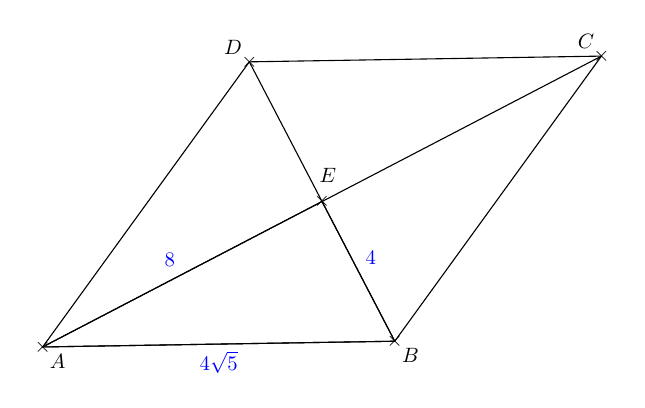
\begin{tikzpicture}[scale=0.5,every node/.style={scale=0.75}]
	%Points
	\begin{scope}[rotate=-62.5]
	\coordinate(A)at(0,0);
	\coordinate(B)at(4,8);
	\coordinate(C)at(0,16);
	\coordinate(D)at(-4,8);
	\coordinate(E)at(0,8);
%	\coordinate(F)at(-1,1);
%	\coordinate(G)at(1,0);
%	\coordinate(H)at(1,1);
%	\coordinate(I)at(2,0);
%	\coordinate(J)at(-1,2);
	\draw (A)--(B)--(C)--(D)--cycle;
	\draw (A)--(C);
	\draw (B)--(D);
	\draw (A)--(E) node[midway, above left, blue]{$8$};
	\draw (B)--(E) node[midway, above right, blue]{$4$};
	\draw (A)--(B) node[midway, below, blue]{$4\sqrt{5}$};
	%Étiquettes
	\foreach \point in {A, B}
		\draw(\point)node{$\times$};
	\foreach \point in {A, B}
		\draw(\point)node[below right]{$\point$};
	\foreach \point in {E}
		\draw(\point)node{$\times$};
	\foreach \point in {E}
		\draw(\point)node[above,shift={(0.1,0.2)}]{$\point$};
	\foreach \point in {C, D}
		\draw(\point)node{$\times$};
	\foreach \point in {C, D}
		\draw(\point)node[above left]{$\point$};
%	\foreach \point in {H}
%		\draw(\point)node{$\times$};
%	\foreach \point in {H}
%		\draw(\point)node[above right]{$\point$};
	\end{scope}
\end{tikzpicture}
%}
\end{center}
\end{minipage}
\begin{minipage}{0.2\textwidth}
Le parallélogramme ci-contre est-il un losange~?
\end{minipage}


\exercice\\

$ABC$ est un triangle isocèle en $A$.\\
Le cercle $\mathscr{C}$ , de diamètre $[AB]$, coupe $[BC]$ en $D$ et $[AC]$ en $E$.\\
La perpendiculaire à $(AB)$ passant par $C$ coupe la droite $(BE)$ en $F$.\\

\textbf{Objectif :} Démontrer que $A$, $D$ et $F$ sont alignés, et que $(AF)$ est la médiatrice de $[BC]$.\\

\begin{enumerate}
	\item Faire une figure.
	\item	\begin{enumerate} 
				\item Quelle est la nature des triangles $AEB$ et $ADB$~?
				\item Pourquoi peut-on affirmer que $F$ est l’orthocentre du triangle $ABC$~?
				\item Pourquoi peut-on affirmer que $(AD)$ est la médiatrice de $[BC]$~?
			\end{enumerate}
	\item	\begin{enumerate} 
				\item Montrer que $(AF)$ et $(BC)$ sont perpendiculaires.
				\item En déduire que $A$, $D$, et $F$ sont alignés, puis que $(AF)$ est médiatrice de $[BC]$.
			\end{enumerate}
\end{enumerate}

\exercice

Les diagonales d’un quadrilatère $ABCD$ se coupent en $E$.

$I$, $J$, $K$, $L$ sont les milieux respectifs de $[AB]$, $[BC]$, $[CD]$, $[DA]$.

\begin{enumerate}
	\item Faire une figure en y reportant toutes les informations de l’énoncé.
	\item Démontrer que $IJKL$ est un parallélogramme.
\end{enumerate}